\chapter{Artificial Intelligence in Video Games}
\label{chap:games}

In video games the implementation of artificial intelligence (AI) is generally constrained most heavily by performance. Maintaining the illusion of a virtual world requires an AI agent to react within a time frame that is reasonable for a human player. Turn-based strategy games like chess or checkers are less impaired by performance because human players are often expected to take long periods of time to make a decision; however, real-time games generally require decisions to be made in milliseconds, severely limiting the complexity of the AI algorithm used. This chapter will provide a brief look at common AI techniques using concrete examples.

\section{Pac-Man}

Early computer controlled video game agents relied primarily on scripting and randomization. Scripting is a process by which a developer manually creates a set of a rules which govern an agent's actions. Randomization was often included in these rules to increase the difficulty of determining how the agent would behave, as well as to mimic human behavior which does not always follow strict rules. A famous example is Pac-man, which made clever use of scripted AI in order to create the illusion that each enemy possessed a different personality \cite{pacman}.

Pac-Man is a game in which the player controls a hungry character, known as the pac-man, who must navigate a maze in order to eat \emph{food} while avoiding enemies called \emph{ghosts}. The ghosts are controlled by the computer and their goal is to kill the player by touching him. They have limited speed and pac-man can consume a special item to make the ghosts vulnerable to attack for a short period of time. Over the years fans of the game Pac-Man have studied and dissected the behavior of the ghosts and published these results as ``The Pac-Man Dossier'' \cite{pacman}. This dossier goes into great detail about the behavior of the ghosts with the intent of allowing players to exploit weaknesses in their behavior.

Each ghost was given a unique set of rules to guide them, resulting in behavior that many players see as resulting from different personalities. One of the ghosts, named Blinky, was programmed to always move toward the space currently occupied by the player. As a result, this ghost was seen as more aggressive and was more likely to kill the player than the other ghosts. Another ghost, called Pinky, was programmed to always target a space in front of the player's direction of movement.

In addition to each ghost's unique movement rules, all ghosts were subject to global rules which helped to prevent the player from being hunted relentlessly. Periodically the ghosts would switch between a chase mode, during which their unique rules were in place, and a scatter mode, during which each ghost would flee to a pre-configured path.

The rules controlling the ghosts in Pac-Man can be trivially represented with conditional statements. This is the signature of scripted AI: simple, fast, and easy to control. For these reasons, scripted AI remains prevalent to this day and often serves as the building block for more complex techniques.

\section{Quake III}
\label{chap:games:quake}

Quake III is a video game in the genre of first person shooters (FPS). In Quake III the player controls a humanoid character fighting against opposing humanoids, called \emph{bots}, in arena-style combat. All players, human or bot, can pick up different weapons which each have different characteristics. Weapons spawn in pre-defined locations on the map as well as other items such as ammunition, health, and armor. Increasing health and armor improves a character's ability to survive attacks from an opponent. Each time a character dies they respawn with a default weapon and stat levels which can be improved by collecting items on the map. The goal is to kill your opponents until you reach a pre-defined kill count which signifies victory. 

The environment for Quake III is orders of magnitude more complex than that of Pac-Man. In Quake III the world is continuous, three dimensional, governed by physics which approximates reality, and the bots were designed as a stand-in for human opponents. To meet this challenge, a more complex AI system than just scripting was required. The designer of this AI, J.M.P van Waveren, designed a hierarchical system which relied on finite state machines for efficient decision making and combined this with fuzzy logic to provide unique personalities \cite{q3bot}.

\begin{figure}
	\centering
		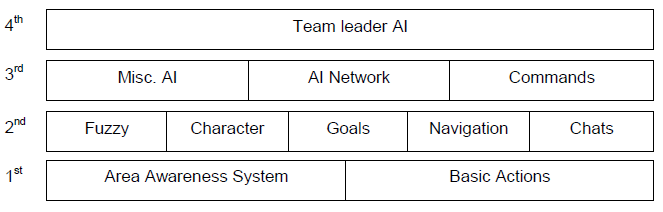
\includegraphics[width=0.80\textwidth]{q3_layers.png}
	\caption{The Quake III AI layers. \cite{q3bot}}
	\label{fig:q3:layers}
\end{figure}

The core of the Quake III bot is composed of four levels, as shown in Figure \ref{fig:q3:layers}. At the lowest level exists the area awareness system (AAS) and the basic actions interface. The AAS provides feedback on the physical state of the world around the bot, such as items or enemies which are visible. The basic actions interface provides a translation of bot commands into the same keyboard inputs a human player uses.

The second level is separated into sections for handling navigation, chat, and bot preferences. This level feeds into the third level, which directs goal-seeking behavior as well as logic to support chat commands and team communication. The fourth level is responsible for coordination between team members.

Breaking the AI design into these levels and sections drastically reduces the complexity of creating a competitive bot. Each of these sections can be designed using very simple decision making structures, but the end result is a bot which was capable of competing with the average human and even coordinating in groups. Most of these sections were implemented as straightforward conditional scripts, with two notable exceptions: the bot preference system and the \emph{AI Network}.

\subsection{Bot Preference}

The bot preference system was implemented in order to allow different bots to have different personalities. Imagine you wanted to implement a bot, Rocky, who has a particular affinity for the rocket launcher. A first attempt might simply have Rocky always go for the rocket launcher. Now imagine how Rocky would perform on a large map, if he spawned in a location such that he needed to cross the entire map in order to reach the rocket launcher. In this scenario, Rocky would have a high risk of being intercepted on the way to the rocket launcher. At this point it would become difficult for him to decide what items to pick up and what weapon to use if he decides to fight. You could start scripting the AI to handle this, but with an extremely large number of scenarios to handle scripting quickly becomes an impossible solution.

To get around this problem, Waveren implemented a fuzzy logic system \cite{q3bot}. Fuzzy logic assumes all values have some continuous truth, rather than just \emph{true} or \emph{false}. This system allows for a lot more granularity in goal selection. Going back to the previous example, rather than simply programming Rocky to go for the rocket launcher, Rocky would be given a high preference for the rocket launcher. To fully flesh out his personality, you would need to fill in his preference for other weapon types, as well as some other characteristics which would determine how likely he is to run from a fight when he does not have the upper hand.

Once Rocky's preferences are filled out, he can then make decisions based on the state of the environment and his own preferences. Now when Rocky starts out he will likely head toward the rocket launcher, but this time when he is approached by an enemy he will be capable of selecting a good nearby weapon to fight with before resuming his trek toward the rocket launcher. This preference system provides a very simple way to create a new bot personality without having to modify the code or logic. Another benefit is that Rocky will know how to behave regardless of the map, items available, or number of enemies that approach him, all without needing to set anything more than his preference values.

\subsection{AI Network}

While the preference system handles decisions regarding what weapons to pick up and what weapon to use, the bot still needs to know when it is a good idea to search for items, fight an enemy, or run away. These decisions are handled by the AI Network. Consider again the situation Rocky was in when an enemy intercepted him while he was searching for the rocket launcher. From a high-level perspective, Rocky can choose to fight, run, or pick up a nearby item. Once again, writing conditional scripts to handle this situation would result in complex code that cannot apply to new maps or item layouts.

\begin{figure}
	\centering
		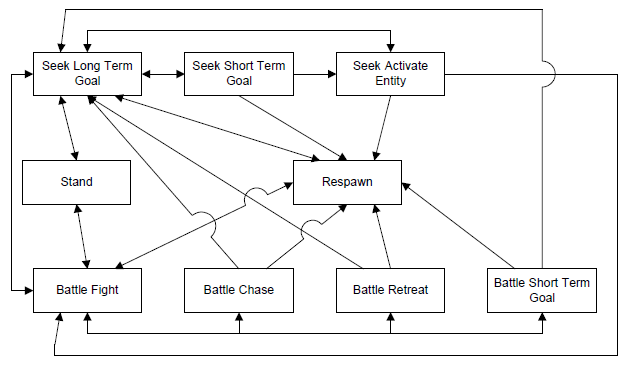
\includegraphics[width=0.80\textwidth]{q3_fsm.png}
	\caption{The Quake III AI Network. \cite{q3bot}}
	\label{fig:q3:fsm}
\end{figure}

Instead of conditional scripts, Waveren implemented the AI Network using a finite state machine as demonstrated in Figure \ref{fig:q3:fsm} \cite{q3bot}. A finite state machine consists of a number of nodes, called  `states', and edges which guide transitions between states. Rocky starts in an initial state called `Seek Long Term Goal'. In this state Rocky uses his preferences and some knowledge of the map to select a long term goal; in our scenario, that would be the rocket launcher. 

As Rocky moves around the map he evaluates the state and checks if anything matches the conditions specified on a transition from the long term goal state. If Rocky runs into an enemy, he would see there is a transition from `Seek Long Term Goal' to `Battle Fight'. Once Rocky is in this state, the transitions available to him change, as do the states he can transition into. 

On its own the finite state machine does not provide a generic decision making process, it just lowers the complexity of the implementation. However, the AI Network transitions are guided by bot preferences, generalizing the decision making process. Between the AI Network and the bot preferences, the Quake III bot provides a strong foundation for a general-purpose AI which is capable of acting in a wide variety of environments without any the need for environment specific logic.

\section{F.E.A.R.}

When F.E.A.R. was under development, the expectations for realistic bot behavior in FPS games was on the rise. Traditional techniques, such as the finite state machine in Quake III, were still resulting in complex and unmanageable behavior. In an attempt to curtail the increasing complexity, the development team decided to use planning algorithms.

A planning system works by defining a goal and a set of actions, then using an algorithm which determines what series of actions will reach that goal. Each action can be represented as a set of prerequisites and expected results. For example, the action $FireWeapon$ might have the prerequisite $WeaponEquipped \land HaveAmmo$ and the expected result $EnemyDead$.

Imagine Rocky is once again searching for a rocket launcher. When Rocky enters a room he sees an enemy at the other side of the room. Rocky checks and finds that $EnemyDead$ is a goal, and that $WeaponEquipped$ is true but  $HaveAmmo$ is false. Luckily for Rocky, a stash of ammunition is nearby and he has the action $PickupAmmo$, which has the prerequisite $AmmoNearby$ and the effect $HaveAmmo$. Rocky then plans to execute the action $PickupAmmo$ followed by $FireWeapon$. Because $FireWeapon$ does not guarantee the effect $EnemyDead$, Rocky will repeat $FireWeapon$ until he kills the enemy.

What happens if Rocky's enemy then runs? Obviously the plan Rocky formed is no longer valid. In this situation, Rocky can then re-evaluate the state of his environment and formulate a new plan to reach his goals.

F.E.A.R.'s planning system reduced the complexity of implementing well-behaved AI by decoupling decision making from the environment. To create a bot, only the actions available to the bot and the goals are needed, the remainder is handled by the planning algorithm. In addition, because the plan and state transitions are dynamically determined, the bot is capable of behavior that is not directly programmed. The end result of this system was a bot which was universally applauded for realistic, tactical bots.

\section{Reinforcement Learning in Video Games}

In the paper ``Learning Agents in Quake III'' researchers from University of Utrecht applied Q-learning to a neural network in order to train combat movements \cite{q3combat}. Neural networks are data structures used to control agent policies by using layers of nodes, each of which takes in an input, processes it, and passes the output to the next layer of nodes \cite{norvig}. Q-learning is an online reinforcement algorithm which was used to learn the optimal weights for each node \cite{norvig}.

The resulting bot was capable of defeating an identical opponent by using superior combat movements in $65\%$ of matches. However, in order to achieve these results they were required to place some restrictions on the environment: the bot was restricted to a single weapon, the room could not have any corners, and there were no obstacles. Additionally, learning the optimal weights required approximately $10$ hours of playtime. While their results were promising, the techniques they proposed are more suitable to generating a policy before letting a user play the game, rather than allowing the bot to develop better techniques while a user is playing.

In 2010, researchers Purvag Patel, Norman Carver, and Shahram Rahimi demonstrated Q-learning in a simulated FPS environment \cite{game:ai:learning}. They created a simulated environment based on the game Counter-Strike for their experiments. First they created a static AI bot which would patrol the map and then they implemented a Q-learning bot designed to learn policies to complete specific tasks, such as killing the enemy or dropping an item at a particular location.

The Q-learning bot randomly selected a patrol route and periodically checked the state to decide if it should start attacking. Further experiments were run with more complicated actions available. The result was an agent capable of learning near optimal policies after only a few thousand samples. While encouraging, because this experiment was done in a simplified and simulated environment, it is difficult to judge how effective the techniques would be when applied to the actual Counter-Strike environment.

Researchers at Lehigh University used Q-learning to generate team coordination policies for agents in the FPS Unreal Tournament, an algorithm they called RETALIATE \cite{retaliate}. The individual bots on all teams followed the same scripted behavior in order to ensure the only variable in performance was the team strategy. In addition to the RETALIATE team, they implemented three scripted teams and a team which used a technique called Hierarchical Task Network (HTN). The HTN team used dynamic planning techniques to develop their policy.

Within a single match, RETALIATE was able to easily learn policies which could defeat the scripted bots. The HTN bot proved more difficult to defeat, but RETALIATE was capable of learning an optimal policy after only two matches.

Our work differs from these experiments primarily in that it evaluates an agent executing in the Quake III environment without utilizing any simulations or restricted environments. In addition, our proposed algorithm uses the GPU to improve performance.